\chapter{Photonic Molecules \label{cap:molecules}}
The technique of writing waveguides using ultrashort laser pulses, described in Chapter~\ref{cap:fs}, allows for the three-dimensional fabrication of photonic structures with micrometric precision. However, this technique has inherent limitations due to the elliptical shape of the laser focus, which imposes restrictions on the transverse modes that can be efficiently excited and, in particular, on the possible intermodal couplings between modes of different symmetry, such as $S$ and $P$ \citep{interorbital}.

To overcome these restrictions and expand the degrees of freedom in the design of photonic networks, an approach inspired by molecular physics is adopted here: by positioning two waveguides sufficiently close, their modes can couple coherently, generating new extended collective modes. This process is analogous to molecular formation in quantum physics, where two atomic orbitals combine linearly to form bonding and antibonding molecular orbitals (see Figure \ref{fig:molec-anal}).

In this work, we will call a \textit{photonic molecule} a system of two coupled waveguides, whose eigenfunctions combine to generate symmetric and antisymmetric hybrid modes, in analogy with molecular orbitals. This analogy is based on the spatial shape of the modes and their controlled overlap, but does not imply the existence of bonding forces, shared electrons, or interatomic potentials. The relationship with quantum molecules is, therefore, formal and geometric, and is restricted to the structural parallelism between optical modes and orbitals \citep{molecules}.

\begin{figure}[H]
	\centering
	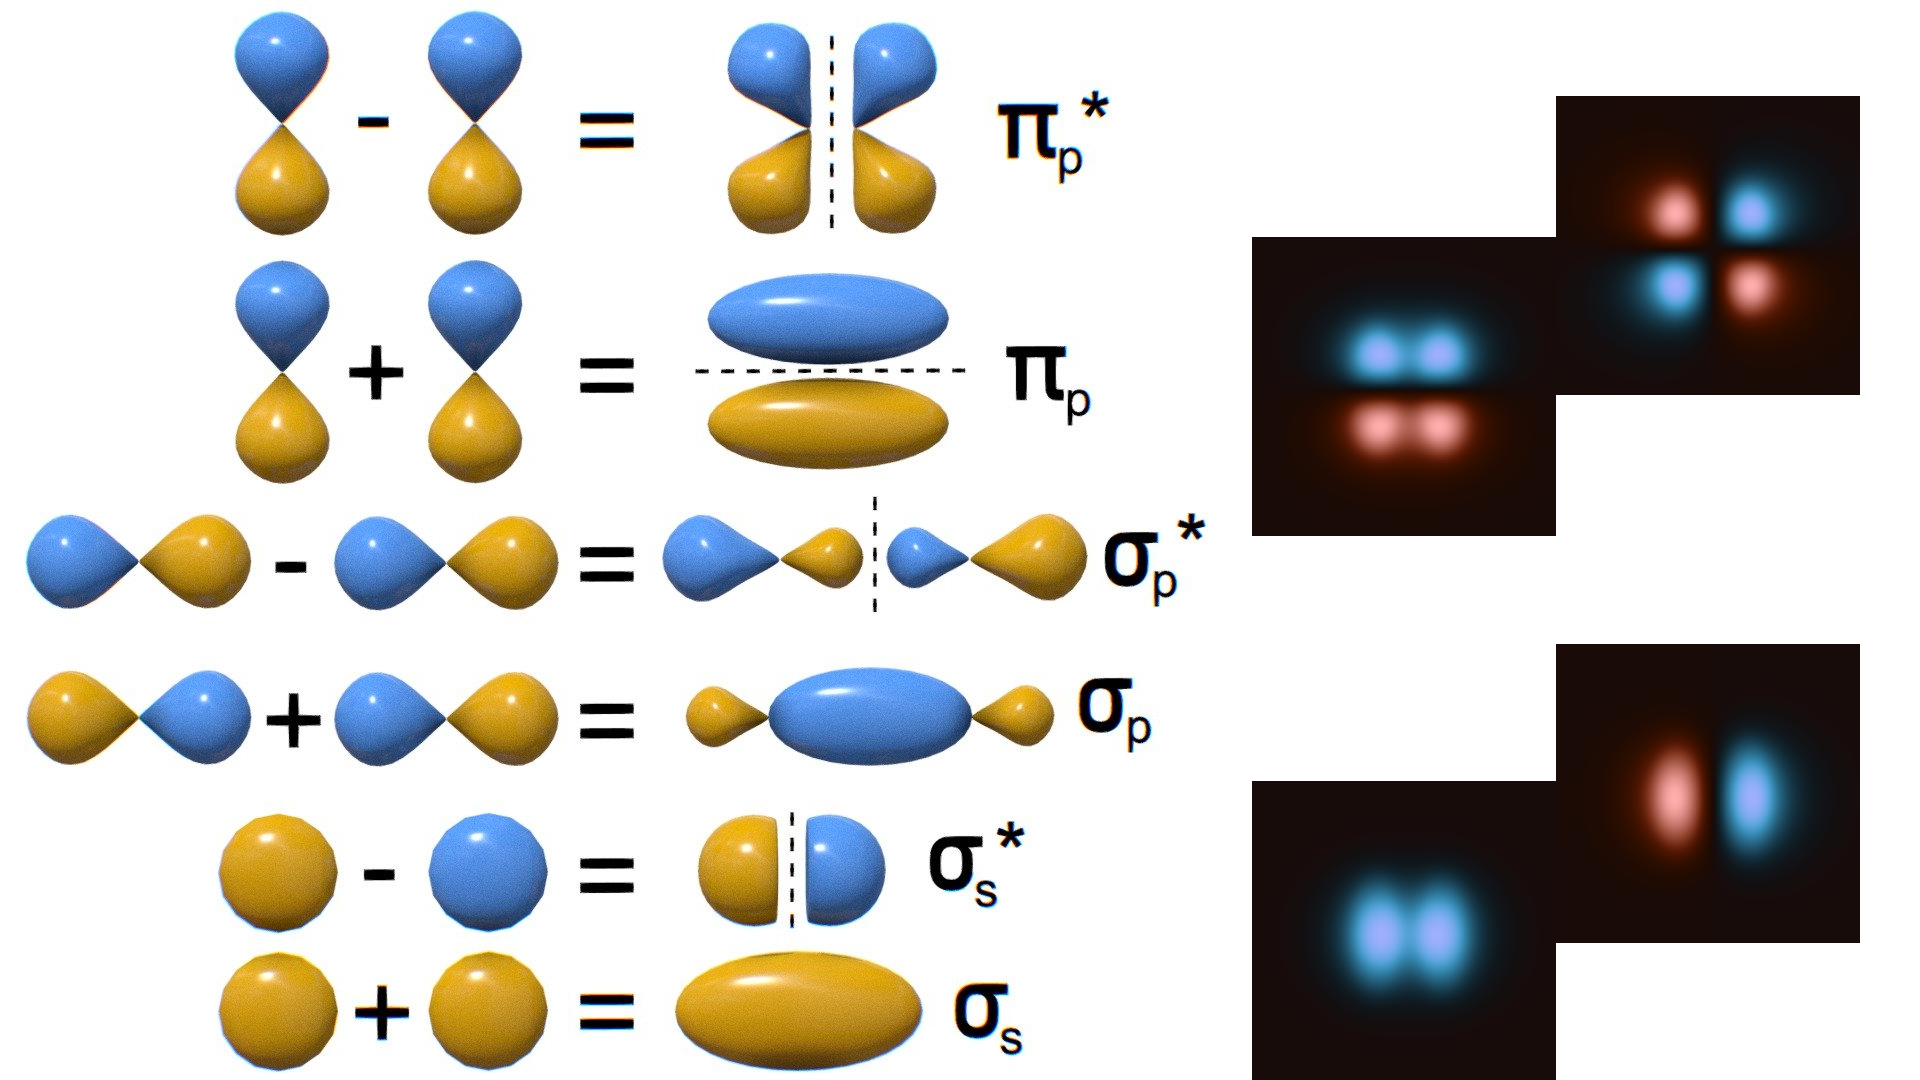
\includegraphics[width=0.6\linewidth]{media/moleculas.png}
	\caption[Analogy and differences between quantum molecules (left) and photonic molecules (right).]{Analogy and differences between quantum molecules (left) and photonic molecules (right). Both atomic orbitals and individual waveguide modes can hybridize, generating new collective states. In the photonic case, hybridization occurs between guided optical modes. Here, there is no photonic analogue of the $\sigma_p$ molecular orbitals. \label{fig:molec-anal}}
\end{figure}

Building on this idea, this chapter experimentally analyzes a photonic lattice constructed from such molecules as basic building blocks. In particular, a periodic SSH-type lattice \citep{SPSSH} is studied—a multi-orbital extension of the Su-Schrieffer-Heeger model—which allows exploring the impact of interorbital $S\hspace*{-0.3ex}P$ coupling on band topology. The system exhibits two independent topological transitions, associated with the modulation of geometric dimerization and the detuning between modes of different symmetry. These transitions are characterized through the observation of edge modes, the calculation of bulk polarization, and spectral analysis, enabling access to a rich photonic phenomenology based on modal engineering.

\section{Eigenstates of the Photonic Coupler for Small Separation Distances}

As mentioned in Section~\ref{cap:CMT}, coupled-mode theory (CMT) adequately describes the photonic systems under study when the distance between waveguides exceeds $13\,\mu$m. or smaller separations, the system must be treated as a single macro-waveguide. The eigenmode expansion (EME), presented in Section~\ref{cap:eme}, provides a numerical tool valid for both regimes. Through simulations of waveguide pairs at different distances, the behavior of their eigenstates was characterized. Figure~\ref{fig:molecule-coup} shows that the antisymmetric eigenstate ($+-$) only exists for distances greater than $13\,\mu$m, as below this threshold it becomes a radiation mode ($k_z^{+-} < k_0 n_0$). In contrast, the symmetric eigenstate ($++$) ersists and can be described as a single entity, which in this thesis will be referred to as the \textit{S mode} of the photonic molecule.
\begin{figure}[H]
	\centering
	
\includegraphics[width=0.9\linewidth]{media/eigenvalues_vs_angle.png}
	\caption[Propagation and couplings in photonic molecules]{
		\textbf{Left:} Propagation constants and couplings as a function of distance for fundamental modes, calculated using EME.
		\textbf{Right:} Propagation constants of $S$ and $P$ modes as a function of wavelength.
		\label{fig:molecule-coup}}
\end{figure}
Although the propagation constants of the $S$ and $P$ modes in the same molecule exhibit different values, they can be equalized between adjacent molecules by adjusting the refractive index contrast in the waveguides \citep{interorbital, SPSSH}. For example, Figure~\ref{fig:molecule-coup} shows that at $730$\,nm the propagation constants are equalized for $\Delta n_S = 5.200 \times 10^{-4}$ and $\Delta n_P = 10.423 \times 10^{-4}$.

\section{Photonic Molecules in the SP-SSH Lattice}

For the experimental implementation (Section~\ref{cap:fs}) of a lattice exhibiting SP coupling \citep{interorbital, toporusos, SPSSH}, the horizontal $P$ modes from the previous section, obtained through photonic molecules, were used. Precise tuning of the propagation constants of the $S$ ($k_z^S$) and $P$ ($k_z^P$) modes allowed considering a degree of freedom analogous to electron spin (\textit{pseudospin}). The Hamiltonian $H$ of this lattice \citep{SPSSH}, illustrated in Figure~\ref{fig:sp-ssh-model}, is as follows:
\begin{align*}
	H &= \sum_n \left[\frac{\delta\beta}{2} \left( p^*_{n, 1} p_{n, 1} - s^*_{n, 1} s_{n, 1} + p^*_{n, 2} p_{n, 2} - s^*_{n, 2} s_{n, 2} \right) + \varkappa_{ss, 2}s^*_{n, 2} s_{n, 1} - \varkappa_{pp, 2}p^*_{n, 2} p_{n, 1} \right. \\
	&+ \varkappa_{ss, 1} \left( s_{n-1, 2}^*s_{n, 1} + s_{n+1, 2}^*s_{n, 2} \right) - \varkappa_{pp, 1} \left( p_{n-1, 2}^*p_{n, 1} + p_{n+1, 2}^*p_{n, 2} \right) + \varkappa_{sp, 2} \left( s_{n, 2}^* p_{n, 1} - p_{n, 2}^* s_{n, 1} \right) \\
	&+ \left. \varkappa_{sp, 1} \left( s_{n-1, 2}^* p_{n, 1} - p_{n-1, 2}^* s_{n, 1} + s_{n+1, 1}^*p_{n, 2} - p_{n+1, 1}^* s_{n, 2} \right) \right] + \text{c.c.}
\end{align*}

\begin{figure}[H]
	\centering
	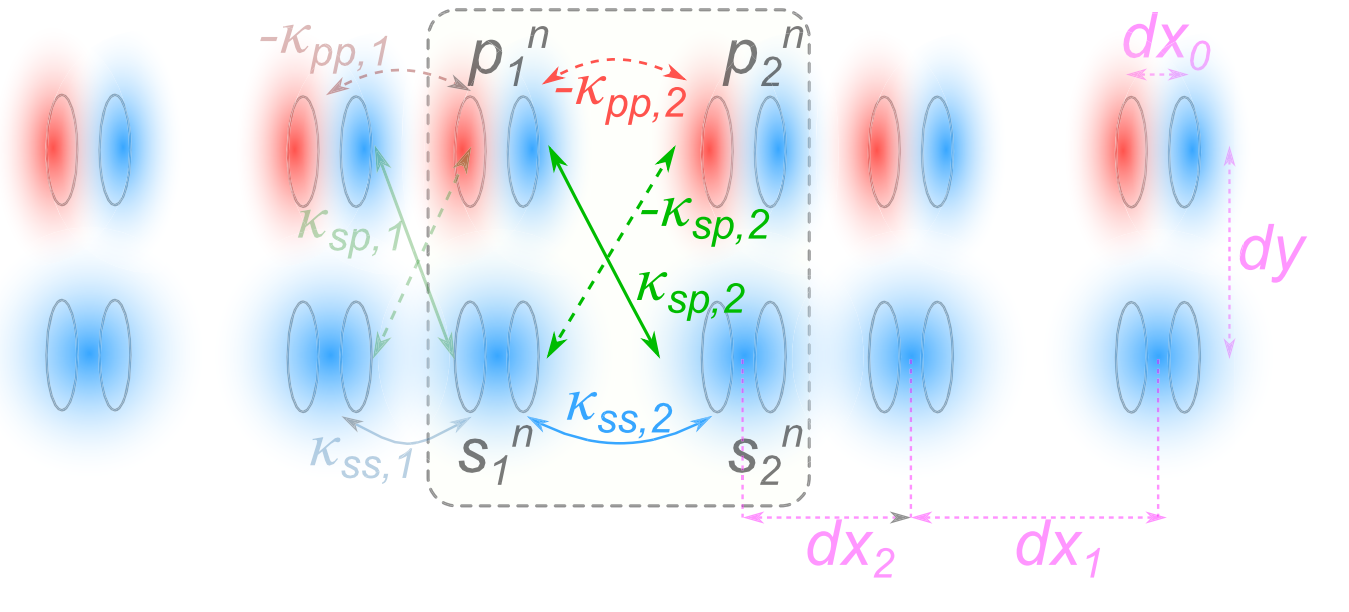
\includegraphics[width=0.7\linewidth]{media/ssh_sp_model}
	\caption{Schematic of the SP-SSH lattice and the considered couplings. \label{fig:sp-ssh-model}}
\end{figure} \vspace{-2ex}
If the basis $\mathbf{v}^n = \left( s_1^n, p_1^n, s_2^n, p_2^n \right)^T$is chosen, the Bloch Hamiltonian can be written in block form as:
\begin{equation*}
	\hat{H}(k) = \begin{pmatrix}
		\hat{\beta} & e^{-ika} \hat{\varkappa}_{1-} + \hat{\varkappa}_{2+} \\
		e^{ika} \hat{\varkappa}_{1+} + \hat{\varkappa}_{2-} & \hat{\beta}
	\end{pmatrix} \ ,
\end{equation*}
donde $\hat{\beta} = \frac{k_z^S - k_z^P}{2} \hat{\sigma}_z$ y $\hat{\varkappa}_{i\pm} = \begin{pmatrix}
	\varkappa_{ss, i} & \pm\varkappa_{sp, i} \\
	\mp\varkappa_{sp, i} & - \varkappa_{pp, i}
\end{pmatrix} \ .$

\section{Topology in the SP-SSH Lattice}
The SP-SSH model allows exploring new topological phases beyond the conventional SSH model, as it incorporates two orbitals ($S$ and $P$ modes) whose linear combinations can be interpreted as a pseudospin. It becomes necessary to study the topology of the system since the spectrum of the Hamiltonian is insufficient to fully explain the behavior of this system, particularly due to the appearance of zero-energy edge states. By applying the unitary transformation
\begin{equation*}
	\hat{U} = \frac{1}{\sqrt{2}}\begin{pmatrix}
		1 & 1 & 0 & 0 \\
		0 & 0 & 1 & -1 \\
		1 & -1 & 0 & 0 \\
		0 & 0 & 1 & 1
	\end{pmatrix} \ ,
\end{equation*} 
it becomes clearer how to interpret the system. In particular, for $\Delta\beta = 0$ and $\varkappa_{ss,1}=\varkappa_{pp,1}$ we have:
\begin{equation*}
	\hat{H} = \begin{pmatrix}
		\hat{H}_+ & 0 \\
		0 & \hat{H}_-
	\end{pmatrix} \ ,
\end{equation*} 
with
\begin{equation*}
	\hat{H}_\pm = \begin{pmatrix}
		0 & e^{-ika}(\varkappa_{ss,1}\mp \varkappa_{sp,1}) + (\varkappa_{ss,2}\pm \varkappa_{sp,2}) \\
		e^{ika}(\varkappa_{ss,1}\mp \varkappa_{sp,1}) + (\varkappa_{ss,2}\pm \varkappa_{sp,2}) & 0
	\end{pmatrix} \ .
\end{equation*}
That is, there are two SSH-type subsystems, with intercell (intracell) coupling $\varkappa_{ss,1}\mp \varkappa_{sp,1}$ ($\varkappa_{ss,2}\pm \varkappa_{sp,2}$).  In the case where $\varkappa_{ss,1}\neq\varkappa_{pp,1}$ it is still possible to capture the topology through the determinant of $\hat{h}=e^{-ika}\hat{\varkappa}_{1-} + \hat{\varkappa}_{2+}$ (ver Figura~\ref{fig:sp-wilson}) (see Figure~\ref{fig:sp-wilson}), since in the complex plane the number of windings around the origin can be counted by sweeping all quasimomenta in the first Brillouin zone. These loops are a generalization of what was shown in Figure~\ref{fig:ssh-topo} regarding the angle formed by the projection in the $xy$ plane of the vector $\mathbf{d}(k)$.

\begin{figure}[H]
	\centering
	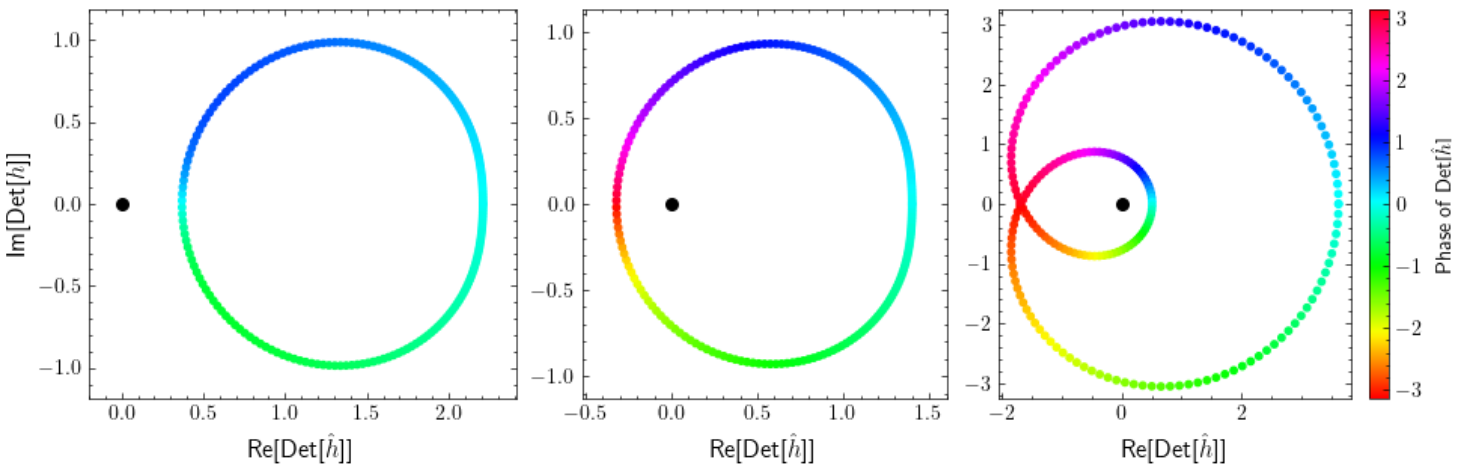
\includegraphics[width=\linewidth]{media/sp-ssh-012.png}
	\caption[Topology of the SP-SSH lattice for $\Delta\beta = 0$.]{Topology of the SP-SSH lattice for $\Delta\beta = 0$. Determinant of the block matrix $\hat{h}$ for quasimomenta $-\frac{\pi}{a} \le k  < \frac{\pi}{a}$. Exactly three distinct topological phases are observed. \label{fig:sp-wilson}}
\end{figure} \vspace{-8ex}
To obtain the full phase diagram (particularly for $\Delta \beta \neq 0$), it is sufficient to vary $\Delta \beta$ and observe when band gap closure occurs, as shown in Figure~\ref{fig:sp-ssh-phase-diagram}. The SP-SSH lattice exhibits two topological mechanisms: one due to SP hybridization and another due to dimerization.
\begin{figure}[H]
	\centering
	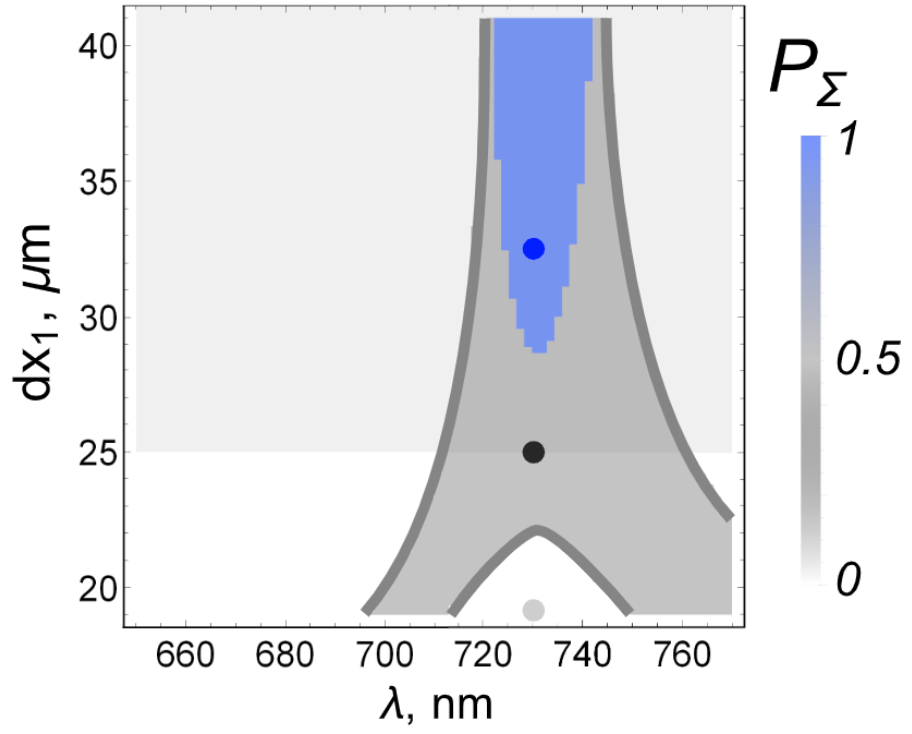
\includegraphics[width=0.6\linewidth]{media/sp-ssh-phase-diagram.png}
	\caption{Topological phase diagram. \label{fig:sp-ssh-phase-diagram}}
\end{figure} \vspace{-2ex}
\section{Experimental Implementation}
To experimentally implement the SP-SSH model, 25 photonic lattices were fabricated using the femtosecond laser writing technique described in Chapter~\ref{cap:fs}. The geometric parameters were adjusted with separations between molecules: variable $dx_1$, $dx_2 = 25$ $\mu$m, $dy = 20$ $\mu$m nd between waveguides: $dx_0 = 7$ $\mu$m. The refractive index contrasts were optimized to achieve mode degeneracy: $k_z^S \sim k_z^P$ at $\lambda = 730$ nm \cite{interorbital}. Measurements were performed via wavelength scanning (Chapter~\ref{cap:wavelength}) with $\lambda \in$ $\{700, 780\}$ nm and a step of 5 nm, aiming to control the parameter $\Delta \beta$, which depends directly on the wavelength used. Excitation was applied to the $S$ waveguide at one end of the lattice, measuring the relative power at the same end ($I_{\text{edge}}/I_{\text{total}}$). Although the topological phases with bulk polarization\footnote{topological invariant that allows distinguishing different topological phases.} $P_\Sigma=1/2$ or $P_\Sigma=1$, are not initially clearly distinguishable, numerical analysis reveals that during the second topological transition the ratio $I_{\text{edge}}/I_{\text{total}}$ should form a plateau. Figure~\ref{fig:sp-ssh-num} confirms this behavior, while Figure~\ref{fig:sp-ssh-exp} shows representative experimental results: one for $\lambda =$ 680 nm, where only dimerization-induced topology is observed, and another for $\lambda =$ 725 nm, where two topological transitions occur as dimerization changes.

\begin{figure}[H]
	\centering
	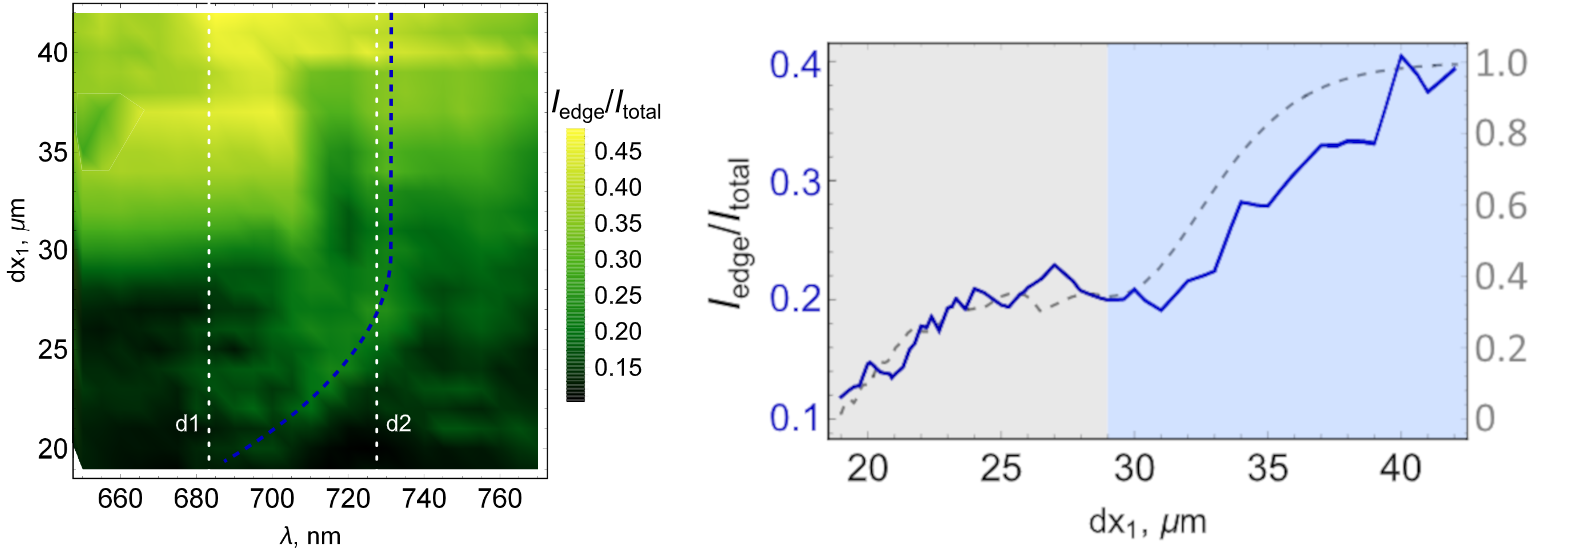
\includegraphics[width=0.9\linewidth]{media/sp-ssh-exp-num.png}
	\caption[Numerical-experimental analysis of the SP-SSH model]{
		\textbf{Left:} Experimental results showing the characteristic plateau.
		\textbf{Right:} Quantitative comparison between experimental data (solid line) and simulations (dashed line).
		\label{fig:sp-ssh-num}}
\end{figure}

\begin{figure}[H]
	\centering
	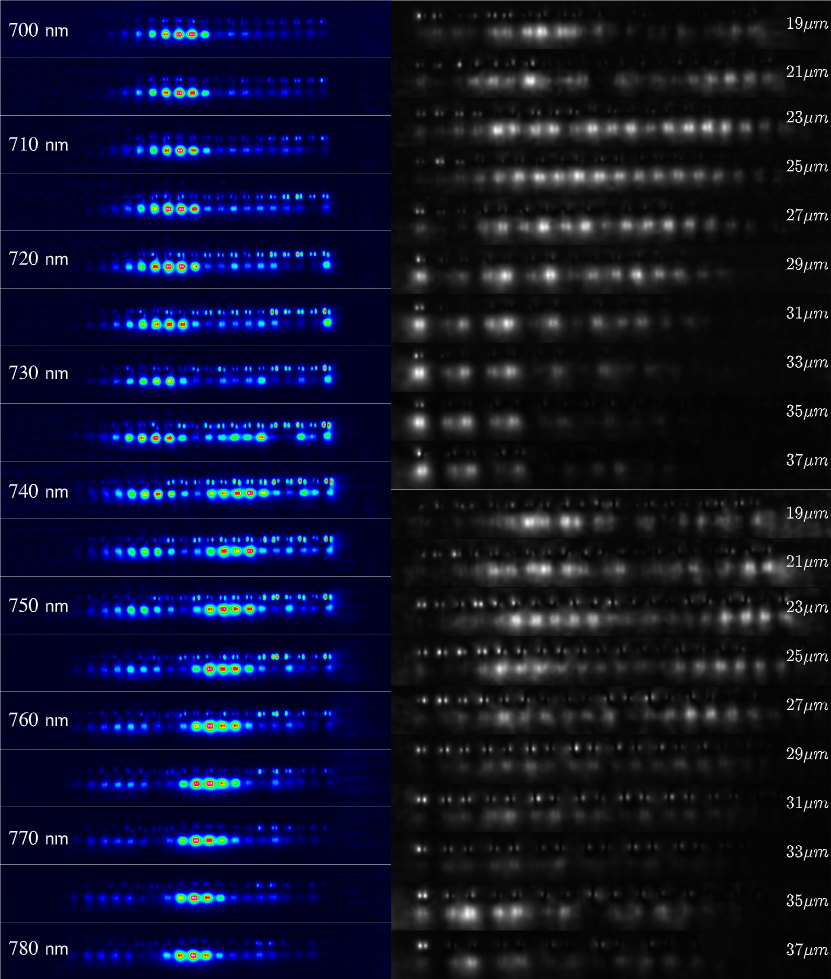
\includegraphics[width=\linewidth]{media/sp-ssh-exp.png}
	\caption[Experimental characterization of SP-SSH lattices]{
		\textbf{Left:} Homogeneous SP-SSH lattice ($dx_1 = dx_2$) for different wavelengths.
		\textbf{Right:} Top: Excitation at 680 nm for different dimerizations.
		Bottom: Same excitation at 725 nm.
		\label{fig:sp-ssh-exp}}
\end{figure}